In this calculator, probabilistic seismic hazard is employed to calculate a
loss exceedance curve for each asset, through the usage of seismic hazard
curves. A convolution between the vulnerability function and the hazard curve
at location of the asset is performed, leading to the probability of exceeding
a set of loss ratios. Each loss ratio is multiplied by the asset value to
obtain the final loss exceedance curve. Furthermore, probabilistic loss maps
can be extracted by interpolating the loss curves at each location by various
probabilities of exceedance. Unlike what was described in the previous
calculator, a total loss curve (considering all assets in the exposure model)
can not be extracted using this calculator, as the correlation of the ground
motion residuals and vulnerability uncertainty is not taken into
consideration. The input and output files involved in this calculator are
presented in Figure~\ref{fig:io-structure-classical-risk}.

\begin{figure}[ht]
\centering
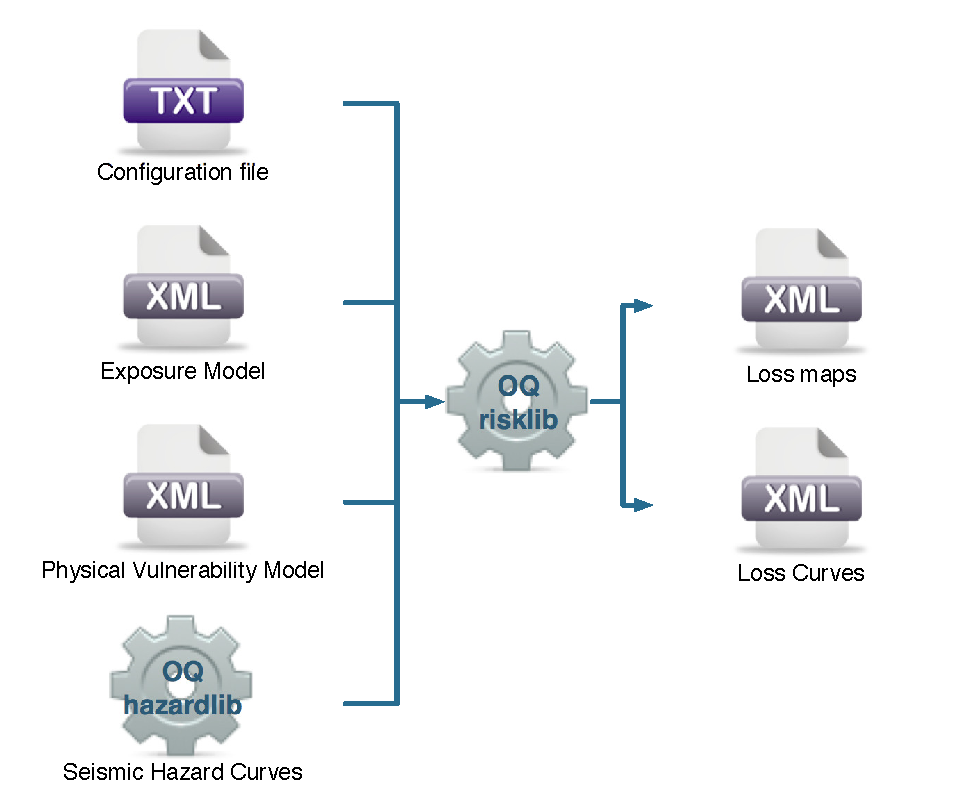
\includegraphics[width=9cm,height=7cm]{figures/risk/io-structure-classical-risk.pdf}
\caption{Classical PSHA-based Risk Calculator input/output structure.}
\label{fig:io-structure-classical-risk}
\end{figure}